%--------------------------------------------------------------- %
\documentclass[SPC-MASTER.tex]{subfiles}
\begin{document}
	\Large
	
\section{Loss Function Analysis}
\begin{itemize}
\item The Taguchi Loss Function is graphical depiction of loss developed by the Japanese business statistician Genichi Taguchi to describe a phenomenon affecting the value of products produced by a company. 
\item Praised by Dr. W. Edwards Deming (the business guru of the 1980s American quality movement),it made clear the concept that quality does not suddenly plummet when, for instance, a machinist exceeds a rigid blueprint tolerance. Instead "loss" in value progressively increases as variation increases from the intended condition. 
\item This was considered a breakthrough in describing quality, and helped fuel the continuous improvement movement that since has become known as lean manufacturing.
\end{itemize}


\begin{figure}[h!]
\centering
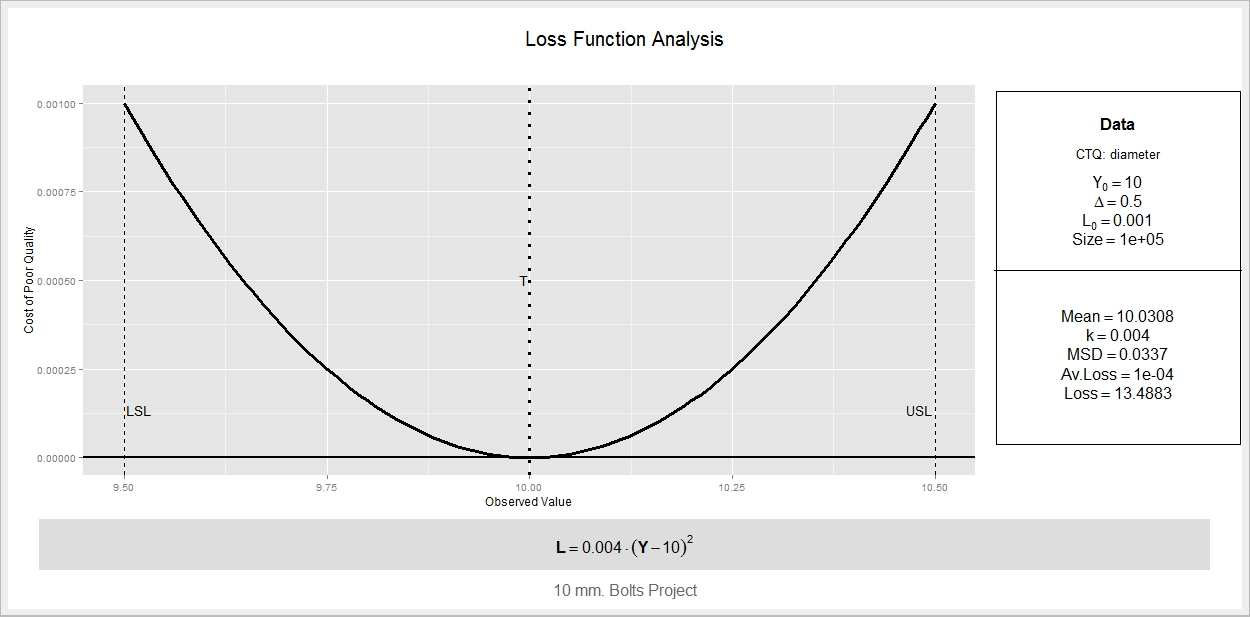
\includegraphics[width=0.99\linewidth]{images/LossFunctionAnalysis}
\caption{}
\label{fig:LossFunctionAnalysis}
\end{figure}
%------------------------------------------------------- %
\end{document}